%       File: VTthesis_template.tex
%     Created: Thu Mar 24 11:00 AM 2016 EDT
%     Last Change: August 15, 2024
%     Author: Alan M. Lattimer, VT
%	  With modifications by Carrie Cross, Robert Browder, and LianTze Lim. 
%
% This template is designed to operate with XeLaTeX.
%
% All elements in the Title, Abstract, and Keywords MUST be formatted as text and NOT as math.
%
%Further instructions for using this template are embedded in the document. Additionally, there are comments at the end of the file that give suggestions on writing your thesis.  
%
%In addition to the standard formatting options, the following options are defined for the VTthesis class: proposal, prelim, doublespace, draft. 

\documentclass[doublespace,nopageskip]{VTthesis} % nopageskip - Removes arbitrary blank pages.
%Remove "draft" from \documentclass to remove draft watermark and to display figures you've created.

% Using the following header instead will create a draft copy of your thesis
%\documentclass[doublespace,draft]{VTthesis}

% The lipsum package is just included to put dummy text in the document in order to demonstrate page headers and table of contents behavior. You should remove it once you begin writing your actual thesis or dissertation.
\usepackage{lipsum}
\usepackage{graphicx}
\usepackage{amsmath}

% Title of your thesis
\title{Optimization of a UAV for Wildfire Management}

% You should include 3-5 keywords, separated by commas
\keywords{Some Keywords, Subject matter, etc.}

% Your name, including middle initial(s)
\author{Nathaniel S. Hargan}

% Change this to your program, e.g. Physics, Civil Engineering, etc.
\program{Mechanical Engineering} 

% Change this to your degree, e.g. Master of Science, Master of Art, etc.
\degree{Master of Science} 

% This should be your defense date:
\submitdate{December XYZ, 2025} 

% Committee members. Only have five readers and one chair available.
% Only use the ones you need and don't include the ones you don't need.
% You can also declare a Co-advisor. Per the VT ETD standards, 
% you should not include titles such as Dr. or Professor, but can list educational 
% qualifications after the name (i.e., John Doe, MFA or Jane Smith, PhD)
% Names should appear as they do in ESS/Banner/HokieSpa, including middle initials.
\principaladvisor{Robert L. West Jr., Ph.D.}
%\coadvisor{Vicente Esparza}
\firstreader{Michael Philen}
\secondreader{Pınar Acar, Ph.D}
% \thirdreader{XYZ}
%\fourthreader{Fourth Committee Member}
%\fifthreader{Fifth Committee Member}

% The dedication and acknowledgement pages are optional. Comment them out to remove them.
% \dedication{This is where you put your dedications.}
% \acknowledge{This is where you put your acknowledgments.}

% The abstract is required.
\abstract{Give a brief description of your thesis here.}
%\abstract{\lipsum [1-4]}

% The general audience abstract is required. There are currently no word limits.
\abstractgenaud{You are also required as of Spring 2016 to include a general audience abstract. This should be geared towards individuals outside of your field that may be reading seeking information about your work. You should avoid language that is particular to your field and clearly define any terms that may have special meaning in your discipline.}

\begin{document}
	% The following lines set up the front matter of your thesis or dissertation and are required to ensure proper formatting per the VT ETD standards. 
	\frontmatter
	\maketitle
	\tableofcontents
	
	% The list of figures and tables are now optional per the official ETD standards.  Unless you have a very good reason for removing them, you should leave these lists in the document. Comment them out to remove them.
	\listoffigures
	\listoftables
	\printnomenclature %Creates a list of abbreviations. Comment out to remove it. 
	
	% sample text for abbreviations:
	NLP is a field of computer science, artificial intelligence, and linguistics concerned with the interactions between computers and human (natural) languages.
	 
	\nomenclature{NLP}{Natural Language Processing}
	
	$\sigma$ is the eighteenth letter of the Greek alphabet, and carries the 's' sound. In the system of Greek numerals, it has a value of 200. 
	
	\nomenclature{$\sigma$}{The total mass of angels per unit area}
	
	% The following sets up the document for the main part of the thesis or dissertation. Do not comment out or remove this line.
	\mainmatter
	
	%now go ahead and start writing your thesis
	\chapter{Introduction} \label{ch:introduction}
	
	%Copy/paste the code below to add sections and subsections to each chapter. Add your own text to the chapter and (sub)section labels to create custom headings.          
	\section{One Section} \label{se:one_section}
	\subsection{A sub-section} \label{ss:this_subsection}
	\section{Another Section} \label{se:another_section}
	
	\chapter{Review of Literature} \label{ch:lit_review}
	
	\chapter{UAV Design} \label{ch:uav_design}
	\section{UAV Geometry} \label{se:uav_geo}
		% General design
		The UAV is modeled as a simplified octocopter frame. [Talk about original UAV design??? [reference???]] The UAV geometry is shown in figure \ref{fig:arm} - figure \ref{fig:hub} with the UAV frame components highlighted. The frame model contains 3 components: the arms, the struts, and the hubs. The arms and struts are both beams with annular cross sections.The hub is two octagonal plates connected with a web shown in figure \ref{fig:hubsec}. The hub model is an simplification, as it can not fit the entire battery within the bounds of hub. Further work can be done to create a more detailed model. 
		
		\begin{figure}[htb]
			\centering
			\includegraphics[scale=0.8]{Images/arm.png}
			\caption{Optimized UAV Model with Highlighted Arm}
			\label{fig:arm}
		\end{figure}
			
		\begin{figure}[htb]
			\centering
			\includegraphics[scale=0.8]{Images/strut.png}
			\caption{Optimized UAV Model with Highlighted Strut} 
			\label{fig:strut}
		\end{figure}
		
		\begin{figure}[htb]
			\centering
			\includegraphics[scale=0.8]{Images/hub.png}
			\caption{Optimized UAV Model with Highlighted Strut} 
			\label{fig:hub}
		\end{figure}
		
		\begin{figure}[htb]
			\centering
			\begin{subfigure}[h]{0.45\textwidth}
				\centering
				\includegraphics[scale=0.8]{Images/hubtop.png}
				\caption{Top View} 
				\label{fig:hubsectop}
			\end{subfigure}
			
			\begin{subfigure}[h]{0.45\textwidth}
				\centering
				\includegraphics[scale=0.8]{Images/hubsectioniso.png}
				\caption{Isometric View} 
				\label{fig:hubseciso}
			\end{subfigure}
			\caption{Optimized UAV Model Hub Cross-section View}
			\label{fig:main_figure}
		\end{figure}
		
		
		% Dimensions and Design variables
		The hub has 3 design variables, the web thickness, the circumscribed hub radius, and the thickness of the plates.  Figure [ref] shows the design variables is[figure showing DVs] The hub height is a parameter set to 64mm as to fit the with UAV battery. [citation needed] 
		% # https://genstattu.com/tattu-40000mah-6s-10c-22-8v-high-voltage-uav-lipo-battery-pack-with-as150-as150-plug/?srsltid=AfmBOoqN5rYTguPKErrR2RGJXuesTt9UqwIoJ9aieuGaF-ipxM2Kz1VW
		
		The arm beams span from the faces of hub to the wingspan. The design variables are thickness and radius. The wingspan is 1127.3mm. It is the minimum length required to fit all 8 propellers with a radius of [440mm??] and a propeller spacing of 25mm.  
		
		The strut beams have 3 design variables, thickness, radius, and, the distance from the hub center to the arm end. Strut deign variables are shown in figure [XYZ fig]. 
		
		The UAV carries a payload of 45kg. All frame components are made from carbon fiber with material properties shown in table [ref XYZ]. [DO I CITE EMAIL? CITATION NEEDED]
		   
		From these design variables relevant cross-section properties are calculated.
		
		The drone batteries are also have a mass of [mass] and dimensions of [dimension]
		
		
il		% My architecture
		The DroneGeometry class within the UAV{\_}Geometry module stores relevant design variables for a drone geometry. The relevant coordinates for hub, arm, and struts are calculated. The projected surface area for drag calculation a drone geometry is calculated using the calc{\_}projected{\_}surfac{\_}area method. [talk about this in detail later]
		
	
		\begin{comment}
		- The UAV is modeled as a simplified version of a UAV frame 

		
		[Talk about the briefly original UAV design (I do not know where to find this)
		
		- Frame designed from 3 components
			- Arms
				- Annulus 
				- Design variables are radius, thickness
				- Arm length runs from the end of the hub to the wingspan
				- the wingspan is the minimum required to fit all propellers with 25 mm of spacing
			- Struts
				- Annulus
				- Design variables are radius, thickness, and distance from center 
			- Hub 
				- Two octagonal plates with sides perpendicular to the arm
				- the web runs in between each 
	
				- Flange thickness, web thickness, and Hub radius are design variables.
				
		- They are assumed to be welded together 
					
		- Payload of the UAV is 45 kg
		
		- Material Properties
			- Table of the relevant material properties of dragon plate. 
		
		- Cross Section Properties
			- Table of the relevant cross section properties
		
			- Arm length is assumed to be the minimum allowable length that allows for 50mm of spacing between propellers.
		 	 
		
		- Hub height is determined to be 64mm to allow for clearance of the battery. [battery source]
		
		\end{comment}
	
		
	
	\section{Mission Profile} \label{se:mission_profile}
		% mission profile general
		A model of the mission profile was created to describe a potential mission with continuous position, velocity, and acceleration with respect to time. The mission profile is modeled as a series of mission profile segments. Constraints are put on the position, velocity, and acceleration at the nodes between mission profile segments. The remaining values at the nodes are calculated using basic kinematic equations. At values of time between mission segment nodes, the position, velocity, and acceleration are interpolated using cubic Hermite splines. [citation needed] Acceleration changes linearly with respect to time. 
		
		% The mission profile 
		The mission profile has an initial takeoff period, a climb to an 100 meter altitude, a cruise period where the UAV travels 2000 meters downrange and increases in altitude 10 meters. Then the UAV descends for 20 seconds and then lands. The climb, cruise, and descent periods are each described using two separate cubic Hermite spline intervals to prevent over-defining the mission profile. Figure \ref{fig:xvy} shows the altitude for the mission profile against the down range position. Figure \ref{fig:yvt} shows the altitude over time. Figure \ref{fig:xvt} shows the downrange position with respect to time. Table \ref{tab:profcons} shows the constraints on the mission profile. The duration shows the time between spline intervals. Blank entries are where no constraint was applied. 
		
		\begin{figure}[htb]
			\centering
			
\includegraphics[scale=0.8]{Images/MissionProfile/XvY.png}
			\caption{Downrange Position vs. Altitude}
			\label{fig:xvy}
		\end{figure}
		
		\begin{figure}[htb]
			\centering
			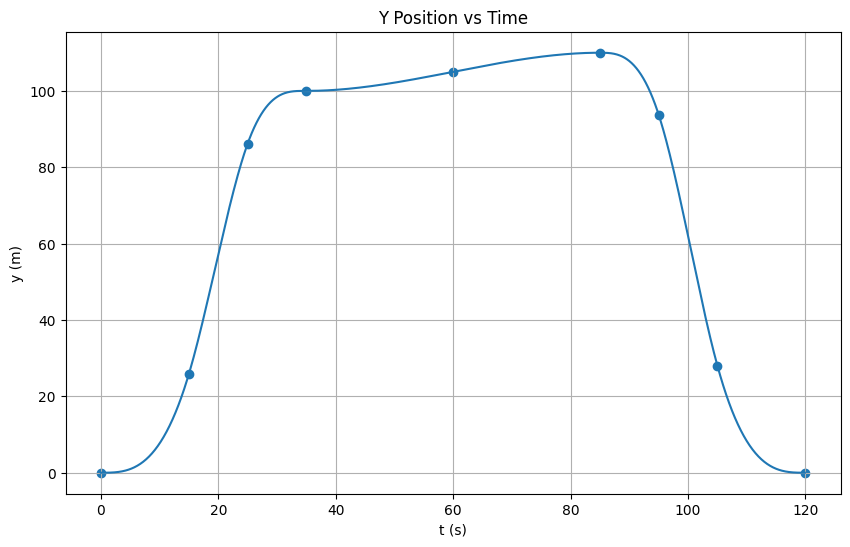
\includegraphics[scale=0.8]{Images/MissionProfile/YposvT.png}
			\caption{Altitude vs. Time} 
			\label{fig:yvt}
		\end{figure}
		
		\begin{figure}[htb]
			\centering
			
\includegraphics[scale=0.8]{Images/MissionProfile/XposVT.png}
			\caption{Downrange position vs. Time} 
			\label{fig:xvt}
		\end{figure}
		

		\begin{table}[htb]
			\centering
			\caption{Mission Profile Constraints} 
			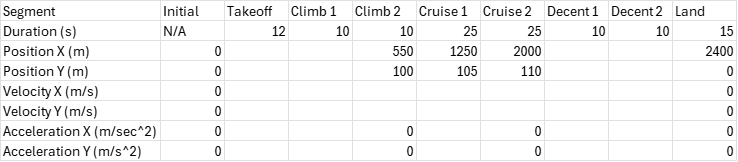
\includegraphics[scale=0.8]{Tables/profcons.png}
			\label{tab:profcons}
		\end{table}
		
		% My specific Architecture
		Mission profiles are generated with a mission{\_}profile module. This module contains a MissionProfile class, MissionProfileSegment class, and the kinematic matrix function. The MissionProfile contains a list of constraints added by the add{\_}constraint method, and a list of segment durations added by the add{\_}segment method. It also contains the solve{\_}kinematics and time{\_}solve method. The solve{\_}kinamatics method assembles matrixes generated from the kinematic{\_}matrix function into a kinematic matrix for the entire mission profile. The remaining position, velocity, and acceleration values at the nodes are then calculated using the numpy.linalg.lstsq function. The time{\_}solve method uses a cubic Hermite spline to find interpolate values at a given time. 
		
		
		
			
	\section{UAV Batteries} \label{se:batteeries}
		
		% https://genstattu.com/tattu-40000mah-6s-10c-22-8v-high-voltage-uav-lipo-battery-pack-with-as150-as150-plug/?srsltid=AfmBOoo89wjweOS5x2-_3PrUxTjnsa3qDuCLy9eYPu2Dz_ErwfbAG77_
		% "battery_mass": 4.292e-3,
		
		% "battery_dimensions": np.array([260.5, 123.5, 63.5]),
		 
		% "battery_volts": 22.8,
		
		% "battery_mah": 40000
		

	
	
	\chapter{Finite Element Analysis} \label{ch:fea}
		
		A finite element model was create to be run repeatedly by the optimization algorithm. 

	
		
		
	\section{Beam Element Formulation} \label{se:beam_element_form}
	
		% Description	
		
		Beams are modeled as timeshenko beams elements with 12 degrees of freedom [citation needed?]. This beam model takes shear deformation effects into account. The mass for each beam is modeled as a 3D lumped mass matrix. Boundary conditions are set relative to a local coordinate system so that the symmetric boundary conditions at the endpoints of the struts. 
		
		% Architecture
		
	
		
		
	\section{Solvers} \label{se:solvers}
		
		An FEA model was crated with three separate solvers. The static solver, which is used to calculate the response given a static loading, the dynamic solver, which calculate thee response given a force of an oscillating force at a given frequency, and the transient solver which calculates the response given a time-changing force. 
		
	\subsection{Static} \label{ss:static}
	
		The static solver uses point loads to 
		- Inputs
			- Point Loads
		- Outputs 
			- Stress 
				- Explain how stress caclualtion is obtained
				- calculated from the local displacment in each element
			- Strain
				- Explain how strain calculation is obtained
				- calculated from the local displacment in each elemen
			- Natural Frequency
				
		
	\subsection{Dynamic} \label{ss:dynamic}
		- Inputs
			- Point Loads
			- Frequency [Cite source]
		- Outputs 
			- Stress Amplitude
			- calculated from the local displacment in each element
		- Strain Amplitude
			- calculated from the local displacment in each element
			- Natural Frequency
	\subsection{Transient} \label{ss:transient}
		- Inputs
			Function describing a force at a given time
		- Uses Newmark integration to calculate resulting transient displacements and reactions
		- The transient stress is obtained from the transient displacements and reactions
	
	
	\section{UAV Segment Model} \label{se:seg_model}
	
	% Description
	A FEA model of single slice of the UAV frame was created. There are symmetric constraints at the midpoints of the strut beams. The center of the UAV is fixed in all 6 degrees of freedom. This assumes that the modes of frequency are symmetric. [maybe write about an asymmetric frequency model if I do that analysis] The arm and struts have an annular cross section. The hub is represented as a series of repeated I-beam cross sections. The width of each I-beam cross-section in the FEA model is the width at the centroid of the corresponding trapezoidal area of the hub.

	
	\begin{comment}
		
		- The FEA model is a single slice of the UAV.
		-
		- This means that only symmetric frequncy modes are considered.
		- Asymmetric modes can be considered in a seperate analysis by crating asymmetrical boundary conditions.  
		- Each beam is defined as an annular cross section.
		- 
		- The width of the cross section is calculate to be the centroid of the trapezoidal section of the octogonal hub being modeeled by the I beam
		
		
		
		
		[include figure]
	\end{comment}
	
	% Archetcture
	The UAV segment model is generated in the DroneFEA class within the drone{\_}fea module. This module requires a DroneGeometry object as input. A BeamSystem object is generated to perform the FEA analysis. The nodes are generated using the create{\_}drone{\_}slice{\_}node method which adds nodes to the BeamSystem object. The  create{\_}drone{\_}slice{\_}beams method calculates the hub section parameters and adds the beams to the BeamSystem object. The boundary{\_}conditions{\_}slice method applies the boundary conditions to the beam model.  
	
	\section{Optimization} \label{se:optimization}
		The problem is formulated as follows:
		$$ \min \textnormal{mass}(d_a,t_a,d_s,t_s,r_s,t_f,t_w) $$
		
		subject to:
		
		$$g_j(x) \le 0; j = 0, 1, 2, ..., J$$
		$$x_i^L \le x_i \le x_i^U$$
		
		design variables: 
		
		\begin{itemize}
			\item $d_a$: arm diameter,
			\item $t_a$: arm thickness,
			\item $d_s$: strut diameter,
			\item $t_s$: strut thickness,
			\item $r_s$: strut distance from center,
			\item $t_f$: hub flange thickness,
			\item $t_w$: hub web thickness 
			\item $h_l$: hub length
		\end{itemize}
		
		derived variables:
		\begin{itemize}
			\item $d_{tip}$: Deflection at tip
			\item $\sigma_{max}$: Maximum stress from bending 
			\item $f_{amp}$: Amplitude of displacement at the tip of the uav arm
			\item $D$: Damage per mission
			\item $ E_{used}$: Energy used over th duration of the mission
			\item $ E_{total}$: Energy used over th duration of the mission
			
		\end{itemize}
		
		design parameters:
		\begin{itemize}
			\item $d_{allowable}$: Deflection allowable
			\item $\sigma_{allowable}$: Stress allowable from bending 
			\item $R_{allowable}$: Allowable amplitude displacement ratio
			\item $n_{missions} $: number of missions before damage
		\end{itemize}
		
		Constraints: \\
		\large
		
		Limit on deflection from bending by force required to lift the UAV. \\
		$$ g_1(d_a,t_a,d_s,t_s,r_s,t_f,t_w,h_l) = d_{tip} \le d_{allowable} $$
		
		Limit on stress from bending by force required to lift the UAV. \\
		$$ g_2(d_a,t_a,d_s,t_s,r_s,t_f,t_w,h_l) = \sigma_{max} \le \sigma_{allowable} $$
		
		
		Limit on amplitude of displacement given a forcing function based on the propeller speed of the UAV. \\
		$$ g_3(d_a,t_a,d_s,t_s,r_s,t_f,t_w,h_l) = \frac{f_{amp}}{d_{tip}} \le R_{allowable} $$
		
		
		Limit on the damage the UAV during a mission. \\
		$$ g_4(d_a,t_a,d_s,t_s,r_s,t_f,t_w,h_l) = D * n_{missions} \le 1 $$
		
		Energy
		$$ g_5(d_a,t_a,d_s,t_s,r_s,t_f,t_w,h_l) = E_{used} / E_{total} \le 0.8 $$
		
		The bounds on design variable were determined by limits on commercially available carbon fiber based on the dragon plate website.  
		
		$$ 9\text{mm} \le r_a \le 50.0\text{mm} $$
		$$ 0.254\text{mm} ≤ t_a ≤ 3.175\text{mm} $$
		$$ 9\text{mm} ≤ r_s ≤ 50.0\text{mm} $$
		$$ 0.254\text{mm} ≤ t_s ≤ 3.175\text{mm} $$
		$$ 400\text{mm} ≤ d_s ≤ 1127.3\text{mm} $$
		$$ 100\text{mm} ≤ h_l ≤ 1127.3\text{mm} $$
		
		% "arm_diameter": (9, 50),
		% "arm_thickness": (0.254, 3.175),
		% "strut_diameter": (9, 50),
		% "strut_thickness": (0.254, 3.175),
		% "strut_distance": (400, 1127.3),
		% "hub_radius": (100, 400),
		% "hub_flange_thickness": (0.7, 12.7),
		% "hub_web_thickness": (0.7, 3.175)
		
		- Optimization algorithm used is SLSQP method using scipi's minimization function.
		   
		
	\subsection{Objective Function and Design Variables} \label{ss:desvar}
	\subsection{Constraints} \label{ss:consts}
	
	\subsubsection{Displacement} \label{sss:displacement}
		- 1/8 of the mass of the frame and playload was modelled as a point load at the end of the UAV arm pointing upward while the center of the UAV is fixed
		- The static solver as used to calculate the maximum displacement magnitude.
		$$ g_1(d_a,t_a,d_s,t_s,r_s,t_f,t_w) = d_{tip} \le d_{allowable} $$
	\subsubsection{Stress} \label{sss:stress}
		- The stress calculation is the same method as the displacement calculation.
		- The allowable stress is deteermined by the maximum stress of the material and a factor of safety. 
		$$ g_2(d_a,t_a,d_s,t_s,r_s,t_f,t_w) = \sigma_{max} \le \sigma_{allowable} $$
	\subsubsection{Frequency} \label{sss:frquency}
		- The goal of the frequency constraint is to make sure that the frequency experienced by the propeller is not near the natural frequency of the vehicle 
		- The dynamic solver is used. 
		- A frequency of 2 * the rad/s of the propeller is used as the propeller has 2 blades.   
		- A force of 1 Neewton is input  at the tip of the UAV bladd
			[frequency plot]
		$$ g_3(d_a,t_a,d_s,t_s,r_s,t_f,t_w) = \frac{f_{amp}}{d_{tip}} \le R_{allowable} $$
	\subsubsection{Damage} \label{sss:damage}
	
	
		- Mission profile with 5s rev up rev down
		- Osciallating force based on propeller freequency 
		- [figurree of oscillating stress]
		- Raincounting
	
	 	% - "mission_count_damage":10000,
		$$ g_4(d_a,t_a,d_s,t_s,r_s,t_f,t_w) = D * n_{missions} \le 1 $$
	\subsubsection{Energy} \label{sss:energy}
		- Mission profile
		- Power to trust calcualtion
		- Battery capacity
		$$ g_5(d_a,t_a,d_s,t_s,r_s,t_f,t_w) = E_{used} / E_{total} \le 0.8 $$
	
	
	
	
	
	
	\chapter{Results} \label{ch:results}
		- The initial guess	were based off of measurements from the original UAV design. 
		- arm diameter, strut diameter, hub radius, flange thickness, and web thickness were all found to converge to boundary conditions
		
	
		% initial_guess = {
		%	"arm_diameter": 50.0,
		%	"arm_thickness": 0.6,
		%	"strut_diameter": 50.0,
		%	"strut_thickness": 0.6,
		%	"strut_distance": 425,
		%	"hub_radius": 100.0,
		%	"hub_flange_thickness": 0.7,
		%	"hub_web_thickness": 0.7
		% }	
		\begin{comment}
		design variables
		arm_diameter: 50.0
		arm_thickness: 0.30233957405287726
		strut_diameter: 50.0
		strut_thickness: 0.3609053941590715
		strut_distance: 556.4454900912388
		hub_radius: 100.0
		hub_flange_thickness: 0.7
		hub_web_thickness: 0.7
		constraints
		deflection: 0.9999999999999993
		stress: 0.977859849282712
		displacement amplitude: 0.29064885956701497
		energy: 0.3260612162830091
		damage: 0.0
		mass w/ payload: 0.8250115057269486 kg
		
		\end{comment}
		
		-Sensitivity analysis 
			- The value of the design variables which did not converge to the boundary conditions were varied by +-0.1\% of thier values to test the optimal solution.   
			\begin{table}[htb]
								\centering
								\caption{}
								\begin{tabular}{ccc}
								
										\midrule
									\end{tabular}
								\label{tab:time_rom}
			\end{table}
	% \chapter{Discussion} \label{ch:discussion}
	\chapter{Conclusions} \label{ch:conclusions}
	
	\chapter{Summary} \label{ch:summary}
	
	% This is the standard bibtex file. Do not include the .bib extension in <bib_file_name>.
	% Uncomment the following lines to include your bibliography: 
	%\bibliography{<bib_file_name>}
	%\bibliographystyle{plainnat}   
	
	% This formats the chapter name to appendix to properly define the headers:
	\appendix
	
	% Add your appendices here. You must leave the appendices enclosed in the appendices environment in order for the table of contents to be correct.
	\begin{appendices}
		\chapter{First Appendix} \label{app:appendix_one}
		\section{Section one} \label{ase:app_one_sect_1}
		\lipsum[1-3]
		\section{Section two} \label{ase:app_one_sect_2}
		\lipsum[1-3]
		\chapter{Second Appendix} \label{app:appendix_two}
		\lipsum[2]
	\end{appendices}
	
\end{document}

\begin{comment}
	
	
	1. Introduction
	a. Overview
	b. Goals and objectives
	c. Scope
	d. thesis outline
	2. Literature Review
	3. Methodology
	a. UAV design
	i. UAV geometry 
	a) octocopter, batteries, payload
	i. free body diagram
	b) wingspan calculation
	c) describe drone_geometry module
	ii. mission profile design
	`	a) define mission profile segments 
	b) demonstrate kinematic constraints used
	c) results
	
	iii. battery and propeller selection
	
	c. finite element model
	i. description of the UAV segment model
	a. describe the boundary conditions, materials ect. 
	ii. beam element formulation
	a) timeshenko beams
	b) boundary conditions
	c) mass matrices
	iii. solvers
	a) static 
	i. outputs stress strain
	a) stress and stain plots of th UAV given the payload
	b) dynamic 
	i. inputs 
	a) description of the loads
	ii. outputs amplitude of the response given a force strain, displacement, reactions, ect.
	c) transient
	i. input 
	a) description of the loads
	ii. outputs reactions and displacements over time. Assumes no damping.
	iv. Results 
	
	d. optimization 
	a. objective function: mass calculation
	
	b. design variables
	i. figure showing design variable measurements
	ii. upper and lower bounds 
	
	c. constraints
	i. displacement
	a) describe force
	b) static solver
	ii. stress (treating like black aluminum)
	a) describe force
	b) static solver
	iii. frequency
	a) constraint formula 	
	b) describe forcing function 
	c) dynamic solver
	iv. damage
	a) constraint formula 	
	b) describe forcing function 
	c) transient solver
	v. energy
	a) constraint formula 
	b) show energy consumption calculation
	
	d. results 
	
	a) plots of the design space
	b) show optimized value and compare it to initial
	5. Summary				
	6. Conclusions
	
	
\end{comment}





%****************************************************************************
% Below are some general suggestions for writing your dissertation:
%
% 1. Label everything with a meaningful prefix so that you
%    can refer back to sections, tables, figures, equations, etc.
%    Usage \label{<prefix>:<label_name>} where some suggested
%    prefixes are:
%			ch: Chapter
%     		se: Section
%     		ss: Subsection
%     		sss: Sub-subsection
%			app: Appendix
%     		ase: Appendix section
%     		tab: Tables
%     		fig: Figures
%     		sfig: Sub-figures
%     		eq: Equations
%
% 2. The VTthesis class provides for natbib citations. You should upload
%	 one or more *.bib bibtex files. Suppose you have two bib files: some_refs.bib and 
%    other_refs.bib.  Then your bibliography line to include them
%    will be:
%      \bibliography{some_refs, other_refs}
%    where multiple files are separated by commas. In the body of 
%    your work, you can cite your references using natbib citations.
%    Examples:
%      Citation                     Output
%      -------------------------------------------------------
%      \cite{doe_title_2016}        [18]
%      \citet{doe_title_2016}       Doe et al. [18]
%      \citet*{doe_title_2016}      Doe, Jones, and Smith [18]
%
%    For a complete list of options, see
%      https://www.ctan.org/pkg/natbib?lang=en
%
% 3. Here is a sample table. Notice that the caption is centered at the top. Also
%    notice that we use booktabs formatting. You should not use vertical lines
%    in your tables.
% 
%				\begin{table}[htb]
	%					\centering
	%					\caption{Approximate computation times in hh:mm:ss for full order 						versus reduced order models.}
	%					\begin{tabular}{ccc}
		%						\toprule
		%						& \multicolumn{2}{c}{Computation Time}\\
		%						\cmidrule(r){2-3}
		%						$\overline{U}_{in}$ m/s & Full Model & ROM \\
		%						\midrule
		%						0.90 & 2:00:00 & 2:08:00\\
		%						0.88 & 2:00:00 & 0:00:03\\
		%						0.92 & 2:00:00 & 0:00:03\\
		%						\midrule
		%						Total & 6:00:00 & 2:08:06\\
		%						\bottomrule
		%					\end{tabular}
	%					\label{tab:time_rom}
	%				\end{table}
% 
% 4. Below are some sample figures. Notice the caption is centered below the
%    figure.
%    a. Single centered figure:
%					\begin{figure}[htb]
	%						\centering
	%						\includegraphics[scale=0.5]{my_figure.eps}
	%						\caption{Average outlet velocity magnitude given an average  
		%				        input velocity magnitude of 0.88 m/s.} 
	%						\label{fig:output_rom}
	%					\end{figure}
%    b. Two by two grid of figures with subcaptions
%					\begin{figure}[htb]
	%						\centering
	%						\begin{subfigure}[h]{0.45\textwidth}
		%							\centering
		%							\includegraphics[scale=0.4]{figure_1_1.eps}
		%							\caption{Subcaption number one}
		%							\label{sfig:first_subfig}
		%						\end{subfigure}
	%						\begin{subfigure}[h]{0.45\textwidth}
		%							\centering
		%							\includegraphics[scale=0.4]{figure_1_2.png}
		%							\caption{Subcaption number two}
		%							\label{sfig:second_subfig}
		%						\end{subfigure}
	%
	%						\begin{subfigure}[h]{0.45\textwidth}
		%							\centering
		%							\includegraphics[scale=0.4]{figure_2_1.pdf}
		%							\caption{Subcaption number three}
		%							\label{sfig:third_subfig}
		%						\end{subfigure}
	%						\begin{subfigure}[h]{0.45\textwidth}
		%							\centering
		%							\includegraphics[scale=0.4]{figure_2_2.eps}
		%							\caption{Subcaption number four}
		%							\label{sfig:fourth_subfig}
		%						\end{subfigure}
	%						\caption{Here is my main caption describing the relationship between the 4 subimages}
	%						\label{fig:main_figure}
	%					\end{figure}
%
%----------------------------------------------------------------------------
%
% The following is a list of definitions and packages provided by VTthesis:
%
% A. The following packages are provided by the VTthesis class:
%      amsmath, amsthm, amssymb, enumerate, natbib, hyperref, graphicx, 
%      tikz (with shapes and arrows libraries), caption, subcaption,
%      listings, verbatim
%
% B. The following theorem environments are defined by VTthesis:
%      theorem, proposition, lemma, corollary, conjecture
% 
% C. The following definition environments are defined by VTthesis:
%      definition, example, remark, algorithm
%
%----------------------------------------------------------------------------
%
%  I hope this template file and the VTthesis class will keep you from having 
%  to worry about the formatting and allow you to focus on the actual writing.
%  Good luck, and happy writing.
%    Alan Lattimer, VT, 2016
%
%****************************************************************************
